\section{EPOC: Endpoint-Preserving Online Correction}
\label{sec:method}

\subsection{Forecasting and feedback order}
Let $t=1,2,\ldots$ index consecutive, nonoverlapping forecast blocks. At the origin of block $t$, a fixed base forecaster maps the preceding $L$ observations to $f_t\in\mathbb{R}^{H\times C}$, where $H$ is the forecast horizon and $C$ is the number of channels. The target $y_t\in\mathbb{R}^{H\times C}$ becomes available only after the block is complete. We define its base residual as
\begin{equation}
 e_t=y_t-f_t.
 \label{eq:base_residual}
\end{equation}
This residual is measured against the uncorrected base forecast, so its definition is independent of the correction issued for block $t$.

Forecast origins advance by $H$ samples. Consequently, $e_{t-1}$ is known when block $t$ is issued, while $e_t$ is not. The correction and its blending weight use only completed blocks. After all of $y_t$ has arrived, the method updates its regression and blending states and retains a summary of $e_t$ for block $t+1$. The experiments use $L=96$ and $H=24$. Figure~\ref{fig:method} shows the information flow and the order of issuance and feedback.

\begin{figure*}[t]
\def\xfigwd{\textwidth}
\centering
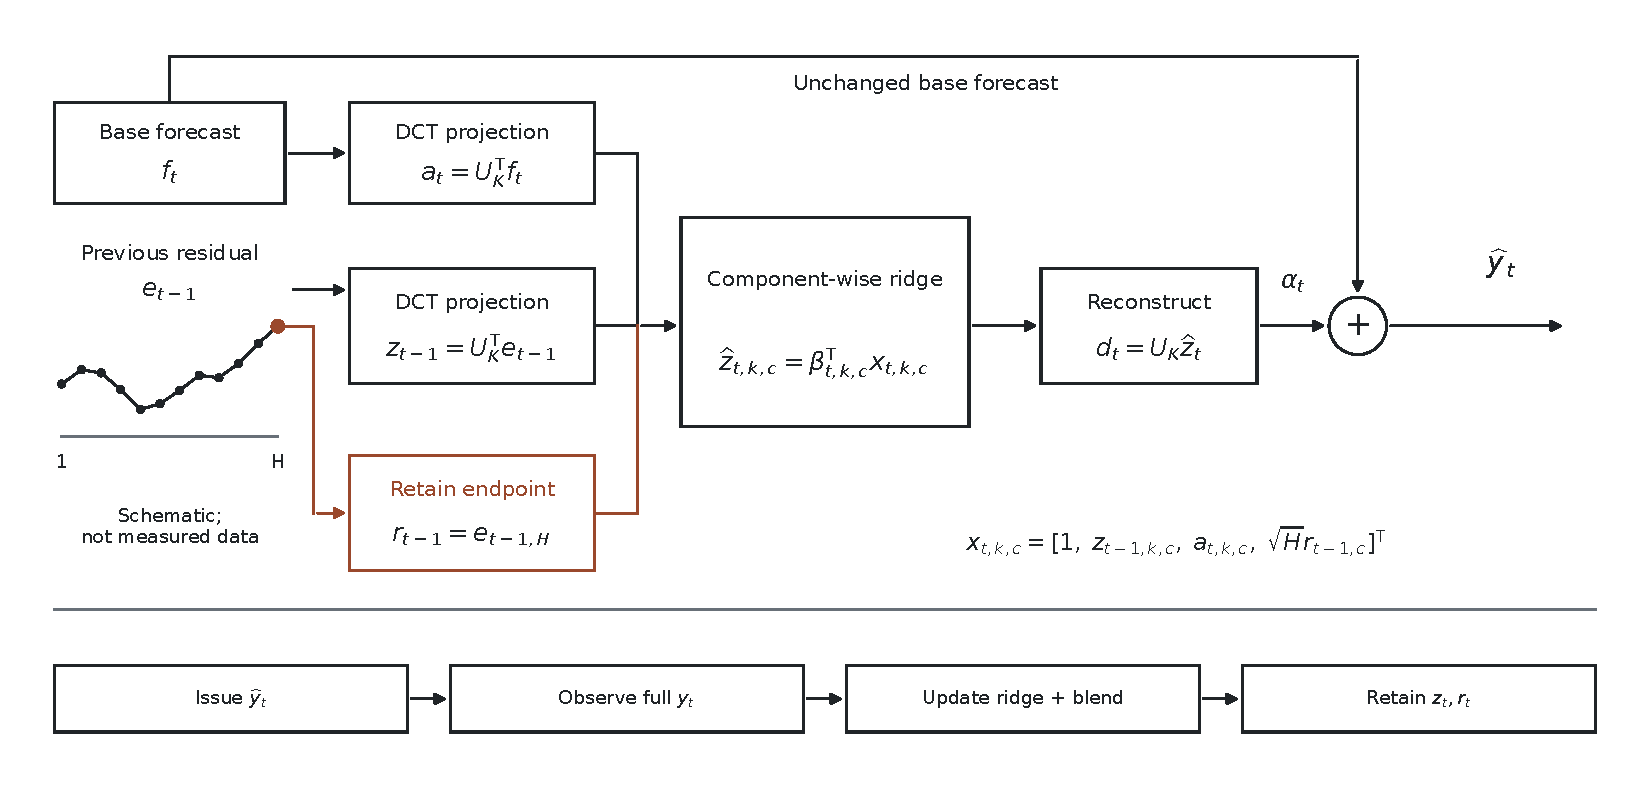
\includegraphics[width=\textwidth]{figure/fig01_method.pdf}
\caption{Correction of block $t$ and the complete-block feedback order. The DCT coefficients and final value of $e_{t-1}$ are available when $f_t$ is issued. The residual trace is schematic. After $y_t$ is fully observed, its base residual updates the regression, the blending controller, and the summary used at the next origin.}
\label{fig:method}
\end{figure*}

\subsection{Residual representation and online correction}
Let $U_K\in\mathbb{R}^{H\times K}$ contain the first $K$ columns of a fixed orthonormal DCT basis~\cite{ahmed1974dct}. The first column is constant. With horizon index $h=1,\ldots,H$ and component index $k=1,\ldots,K$,
\begin{equation}
 (U_K)_{h,k}=\begin{cases}
 H^{-1/2}, & k=1,\\
 \sqrt{2/H}\cos\!\left[\pi(h-\tfrac12)(k-1)/H\right], & k>1.
 \end{cases}
 \label{eq:dct_basis}
\end{equation}
Thus $U_K^{\mathsf T}U_K=I_K$. For channel $c$, we retain the coefficients of the preceding base residual and its observed final value, and transform the current base forecast:
\begin{equation}
 \begin{split}
 z_{t-1,c}&=U_K^{\mathsf T}e_{t-1,c},\qquad
 a_{t,c}=U_K^{\mathsf T}f_{t,c},\\
 r_{t-1,c}&=e_{t-1,H,c}.
 \end{split}
 \label{eq:retained_features}
\end{equation}
The reference configuration uses $K=4$. Before the first evaluated block, $z_{0,c}$ and $r_{0,c}$ are zero.

We estimate each correction component with a separate regression for each channel. Its four-dimensional input is
\begin{equation}
 x_{t,k,c}=\bigl[1,\ z_{t-1,k,c},\ a_{t,k,c},\
 \sqrt{H}\,r_{t-1,c}\bigr]^{\mathsf T}.
 \label{eq:regression_input}
\end{equation}
The same uncompressed endpoint $r_{t-1,c}$ is supplied to all $K$ regressions of channel $c$; it is stored once per channel. The factor $\sqrt H$ is fixed. If the residual is constant throughout a block, the scaled endpoint equals its constant DCT coefficient, so the two inputs have the same scale in that case.

The endpoint can distinguish residual blocks that have the same retained DCT coefficients. Let $\delta_H\in\mathbb{R}^H$ select the final sample and set $v=(I_H-U_KU_K^{\mathsf T})\delta_H$. When $K<H$, $U_K^{\mathsf T}v=0$, whereas $\delta_H^{\mathsf T}v=\lVert v\rVert_2^2>0$. Adding $v$ to a residual block therefore leaves its first $K$ coefficients unchanged but changes its endpoint. This establishes the information difference between the stored endpoint and the endpoint reconstructed from truncated coefficients; their forecasting effect is evaluated in Fig.~\ref{fig:input_ablation}.

For each $(k,c)$, let $\beta_{t,k,c}\in\mathbb{R}^4$ be the coefficients fitted before block $t$. We use exponentially weighted ridge regression~\cite{hoerl1970ridge,goel2020rls} on inputs recorded at their original forecast times:
\begin{equation}
 \begin{split}
 \beta_{t,k,c}=\mathop{\arg\min}_{b\in\mathbb{R}^4}\;&
 \lambda\lVert b\rVert_2^2\\
 &+\sum_{s=1}^{t-1}\rho^{t-1-s}
 \bigl(z_{s,k,c}-b^{\mathsf T}x_{s,k,c}\bigr)^2.
 \end{split}
 \label{eq:ridge_objective}
\end{equation}
The target $z_{s,k,c}$ is the coefficient of the base residual revealed after block $s$. The penalty includes the intercept. We set $\lambda=1$ and $\rho=2^{-1/128}$, giving a weight half-life of 128 completed blocks.

The objective can be updated without retaining previous blocks. With $(k,c)$ suppressed, initialize $G_1=\lambda I_4$ and $q_1=0$. After $y_t$ is observed, update
\begin{equation}
 \begin{split}
 G_{t+1}&=\rho G_t+x_t x_t^{\mathsf T}
 +(1-\rho)\lambda I_4,\\
 q_{t+1}&=\rho q_t+x_t z_t.
 \end{split}
 \label{eq:ridge_update}
\end{equation}
Solving $G_t\beta_t=q_t$ gives the minimizer of~\eqref{eq:ridge_objective}. The final term in the Gram update keeps the ridge penalty fixed while older observations lose weight. The implementation packs the symmetric statistics and solves the linear system directly.

The fitted coefficient, raw correction, and final issued forecast are
\begin{equation}
 \widehat z_{t,k,c}=\beta_{t,k,c}^{\mathsf T}x_{t,k,c},
 \qquad d_t=U_K\widehat z_t,
 \label{eq:raw_correction}
\end{equation}
\begin{equation}
 \widehat y_t=f_t+\alpha_t d_t.
 \label{eq:final_forecast}
\end{equation}
The correction for each channel lies in $\operatorname{span}(U_K)$. The separately retained endpoint changes the regression inputs, while $K$ fixes the correction output dimension.

The scalar $\alpha_t\in[0,1]$ is shared across all horizons and channels. For each completed block $s$, the controller records the squared magnitude of the raw correction and its agreement with the base residual:
\begin{equation}
 A_s=\frac{\lVert d_s\rVert_F^2}{HC},\qquad
 B_s=\frac{\langle d_s,e_s\rangle_F}{HC}.
 \label{eq:blend_statistics}
\end{equation}
Let $\mathcal W_t=\{\max(1,t-W),\ldots,t-1\}$ contain at most $W$ completed blocks. Minimizing the squared error of $f_s+\alpha d_s$ over these blocks for one bounded weight gives
\begin{equation}
 \alpha_t=\begin{cases}
 \operatorname{clip}_{[0,1]}\!\left(
 \dfrac{\sum_{s\in\mathcal W_t}B_s}
 {\sum_{s\in\mathcal W_t}A_s}\right),
 &\sum_{s\in\mathcal W_t}A_s>0,\\
 0,&\text{otherwise}.
 \end{cases}
 \label{eq:blend_weight}
\end{equation}
We use $W=32$. The controller uses the raw correction computed when block $s$ was issued; it does not recompute that correction with later regression coefficients. Algorithm~\ref{alg:online_correction} specifies the issue and update order.

\begin{algorithm}[H]
\caption{Online retained-state correction}
\label{alg:online_correction}
\renewcommand{\algorithmicrequire}{\textbf{Input:}}
\renewcommand{\algorithmicensure}{\textbf{Output:}}
\begin{algorithmic}[1]
\REQUIRE Base forecast $f_t$ at each origin; completed target $y_t$ after issuance; fixed $U_K$, $\lambda$, $\rho$, and $W$.
\ENSURE Corrected forecast $\widehat y_t$ issued before $y_t$ arrives.
\STATE Initialize $z_{0,c}=r_{0,c}=0$, $G_1=\lambda I_4$, $q_1=0$, and an empty controller.
\FOR{each block $t$}
\STATE Receive $f_t$; compute $a_t$, $x_{t,k,c}$, $\widehat z_t$, and $\alpha_t$ from prior state.
\STATE Issue $\widehat y_t=f_t+\alpha_t U_K\widehat z_t$; retain $d_t$ and $x_{t,k,c}$ until feedback.
\STATE After all of $y_t$ arrives, compute $e_t=y_t-f_t$ and $z_t=U_K^{\mathsf T}e_t$.
\STATE Update the controller with $(d_t,e_t)$ and each regression with $(x_{t,k,c},z_{t,k,c})$.
\STATE Retain $z_{t,c}$ and $r_{t,c}=e_{t,H,c}$ for block $t+1$.
\ENDFOR
\end{algorithmic}
\end{algorithm}

\subsection{Retained-state accounting}
We count numerical arrays kept by the correction method between forecast blocks. Its regression statistics contain, for each of the $KC$ regressions, six packed entries of the symmetric Gram matrix for three non-intercept features, three intercept--feature cross terms, and four target cross terms. The intercept weight sum is common to every regression and is stored once. These statistics therefore occupy $13KC+1$ floating-point values.

The other retained arrays contain $HK$ values for $U_K$, $KC$ previous residual coefficients, $C$ endpoints, and $2W+2$ values for the circular blending history and its running sums. The implementation also retains $K$ component indices. All counted values and indices use 64 bits, giving
\begin{equation}
 S(H,K,C,W)=8\bigl(HK+K+14KC+C+2W+3\bigr)
 \ \text{bytes}.
 \label{eq:state_bytes}
\end{equation}
At $H=24$, $K=4$, and $W=32$, this is $8(167+57C)$ bytes: 4,528 B for a seven-channel ETT series, 8,176 B for a 15-channel BDG2 site, and 13,192 B for the 26-channel Appliances series. The median over the 96 fixed-base conditions is 6,352 B, as reported in Table~\ref{tab:main_results}. This is the size of persistent auxiliary numerical arrays. The base forecaster, common observation history, forecast and target buffers, temporary features and solver workspace, and language-runtime overhead are outside this count; it is not a measurement of peak RAM or execution time.
